\documentclass[twoside]{book}

% Packages required by doxygen
\usepackage{fixltx2e}
\usepackage{calc}
\usepackage{doxygen}
\usepackage{graphicx}
\usepackage[utf8]{inputenc}
\usepackage{makeidx}
\usepackage{multicol}
\usepackage{multirow}
\PassOptionsToPackage{warn}{textcomp}
\usepackage{textcomp}
\usepackage[nointegrals]{wasysym}
\usepackage[table]{xcolor}

% Font selection
\usepackage[T1]{fontenc}
\usepackage{mathptmx}
\usepackage[scaled=.90]{helvet}
\usepackage{courier}
\usepackage{amssymb}
\usepackage{sectsty}
\renewcommand{\familydefault}{\sfdefault}
\allsectionsfont{%
  \fontseries{bc}\selectfont%
  \color{darkgray}%
}
\renewcommand{\DoxyLabelFont}{%
  \fontseries{bc}\selectfont%
  \color{darkgray}%
}
\newcommand{\+}{\discretionary{\mbox{\scriptsize$\hookleftarrow$}}{}{}}

% Page & text layout
\usepackage{geometry}
\geometry{%
  a4paper,%
  top=2.5cm,%
  bottom=2.5cm,%
  left=2.5cm,%
  right=2.5cm%
}
\tolerance=750
\hfuzz=15pt
\hbadness=750
\setlength{\emergencystretch}{15pt}
\setlength{\parindent}{0cm}
\setlength{\parskip}{0.2cm}
\makeatletter
\renewcommand{\paragraph}{%
  \@startsection{paragraph}{4}{0ex}{-1.0ex}{1.0ex}{%
    \normalfont\normalsize\bfseries\SS@parafont%
  }%
}
\renewcommand{\subparagraph}{%
  \@startsection{subparagraph}{5}{0ex}{-1.0ex}{1.0ex}{%
    \normalfont\normalsize\bfseries\SS@subparafont%
  }%
}
\makeatother

% Headers & footers
\usepackage{fancyhdr}
\pagestyle{fancyplain}
\fancyhead[LE]{\fancyplain{}{\bfseries\thepage}}
\fancyhead[CE]{\fancyplain{}{}}
\fancyhead[RE]{\fancyplain{}{\bfseries\leftmark}}
\fancyhead[LO]{\fancyplain{}{\bfseries\rightmark}}
\fancyhead[CO]{\fancyplain{}{}}
\fancyhead[RO]{\fancyplain{}{\bfseries\thepage}}
\fancyfoot[LE]{\fancyplain{}{}}
\fancyfoot[CE]{\fancyplain{}{}}
\fancyfoot[RE]{\fancyplain{}{\bfseries\scriptsize Generated on Sun Dec 7 2014 17\+:07\+:27 for A\+N\+Z Task by Doxygen }}
\fancyfoot[LO]{\fancyplain{}{\bfseries\scriptsize Generated on Sun Dec 7 2014 17\+:07\+:27 for A\+N\+Z Task by Doxygen }}
\fancyfoot[CO]{\fancyplain{}{}}
\fancyfoot[RO]{\fancyplain{}{}}
\renewcommand{\footrulewidth}{0.4pt}
\renewcommand{\chaptermark}[1]{%
  \markboth{#1}{}%
}
\renewcommand{\sectionmark}[1]{%
  \markright{\thesection\ #1}%
}

% Indices & bibliography
\usepackage{natbib}
\usepackage[titles]{tocloft}
\setcounter{tocdepth}{3}
\setcounter{secnumdepth}{5}
\makeindex

% Hyperlinks (required, but should be loaded last)
\usepackage{ifpdf}
\ifpdf
  \usepackage[pdftex,pagebackref=true]{hyperref}
\else
  \usepackage[ps2pdf,pagebackref=true]{hyperref}
\fi
\hypersetup{%
  colorlinks=true,%
  linkcolor=blue,%
  citecolor=blue,%
  unicode%
}

% Custom commands
\newcommand{\clearemptydoublepage}{%
  \newpage{\pagestyle{empty}\cleardoublepage}%
}


%===== C O N T E N T S =====

\begin{document}

% Titlepage & ToC
\hypersetup{pageanchor=false,
             bookmarks=true,
             bookmarksnumbered=true,
             pdfencoding=unicode
            }
\pagenumbering{roman}
\begin{titlepage}
\vspace*{7cm}
\begin{center}%
{\Large A\+N\+Z Task \\[1ex]\large 1.\+0.\+0 }\\
\vspace*{1cm}
{\large Generated by Doxygen 1.8.8}\\
\vspace*{0.5cm}
{\small Sun Dec 7 2014 17:07:27}\\
\end{center}
\end{titlepage}
\clearemptydoublepage
\tableofcontents
\clearemptydoublepage
\pagenumbering{arabic}
\hypersetup{pageanchor=true}

%--- Begin generated contents ---
\chapter{Hierarchical Index}
\section{Class Hierarchy}
This inheritance list is sorted roughly, but not completely, alphabetically\+:\begin{DoxyCompactList}
\item \contentsline{section}{com.\+anz.\+mobile.\+anzvolley.\+wrapper.\+Anz\+Volley}{\pageref{classcom_1_1anz_1_1mobile_1_1anzvolley_1_1wrapper_1_1_anz_volley}}{}
\item \contentsline{section}{com.\+anz.\+mobile.\+anzvolley.\+wrapper.\+Anz\+Volley\+Log}{\pageref{classcom_1_1anz_1_1mobile_1_1anzvolley_1_1wrapper_1_1_anz_volley_log}}{}
\item \contentsline{section}{com.\+anz.\+mobile.\+anzvolley.\+wrapper.\+restful.\+Anz\+Volley\+Restful\+Request\+Factory}{\pageref{classcom_1_1anz_1_1mobile_1_1anzvolley_1_1wrapper_1_1restful_1_1_anz_volley_restful_request_factory}}{}
\item \contentsline{section}{com.\+anz.\+mobile.\+anzvolley.\+wrapper.\+restful.\+Anz\+Volley\+Restful\+Response\+Listener$<$ T $>$}{\pageref{interfacecom_1_1anz_1_1mobile_1_1anzvolley_1_1wrapper_1_1restful_1_1_anz_volley_restful_response_listener_3_01_t_01_4}}{}
\item \contentsline{section}{com.\+anz.\+mobile.\+anzvolley.\+wrapper.\+model.\+Earthquake}{\pageref{classcom_1_1anz_1_1mobile_1_1anzvolley_1_1wrapper_1_1model_1_1_earthquake}}{}
\item \contentsline{section}{com.\+anz.\+mobile.\+anzvolley.\+wrapper.\+json.\+Request\+Object}{\pageref{classcom_1_1anz_1_1mobile_1_1anzvolley_1_1wrapper_1_1json_1_1_request_object}}{}
\begin{DoxyCompactList}
\item \contentsline{section}{com.\+anz.\+mobile.\+anzvolley.\+wrapper.\+json.\+Request\+Earthquake}{\pageref{classcom_1_1anz_1_1mobile_1_1anzvolley_1_1wrapper_1_1json_1_1_request_earthquake}}{}
\end{DoxyCompactList}
\item \contentsline{section}{com.\+anz.\+mobile.\+anzvolley.\+wrapper.\+json.\+Response\+Object}{\pageref{classcom_1_1anz_1_1mobile_1_1anzvolley_1_1wrapper_1_1json_1_1_response_object}}{}
\begin{DoxyCompactList}
\item \contentsline{section}{com.\+anz.\+mobile.\+anzvolley.\+wrapper.\+json.\+Response\+Earthquake}{\pageref{classcom_1_1anz_1_1mobile_1_1anzvolley_1_1wrapper_1_1json_1_1_response_earthquake}}{}
\end{DoxyCompactList}
\item \contentsline{section}{com.\+anz.\+mobile.\+anzvolley.\+wrapper.\+restful.\+Anz\+Volley\+Restful\+Request\+Factory.\+Service}{\pageref{interfacecom_1_1anz_1_1mobile_1_1anzvolley_1_1wrapper_1_1restful_1_1_anz_volley_restful_request_factory_1_1_service}}{}
\item \contentsline{section}{com.\+anz.\+mobile.\+anzvolley.\+wrapper.\+Anz\+Volley\+Hurl\+Stack.\+Url\+Rewriter}{\pageref{interfacecom_1_1anz_1_1mobile_1_1anzvolley_1_1wrapper_1_1_anz_volley_hurl_stack_1_1_url_rewriter}}{}
\item Http\+Stack\begin{DoxyCompactList}
\item \contentsline{section}{com.\+anz.\+mobile.\+anzvolley.\+wrapper.\+Anz\+Volley\+Hurl\+Stack}{\pageref{classcom_1_1anz_1_1mobile_1_1anzvolley_1_1wrapper_1_1_anz_volley_hurl_stack}}{}
\end{DoxyCompactList}
\item Json\+Request\begin{DoxyCompactList}
\item \contentsline{section}{com.\+anz.\+mobile.\+anzvolley.\+wrapper.\+restful.\+Anz\+Volley\+Restful\+Request$<$ T $>$}{\pageref{classcom_1_1anz_1_1mobile_1_1anzvolley_1_1wrapper_1_1restful_1_1_anz_volley_restful_request_3_01_t_01_4}}{}
\end{DoxyCompactList}
\end{DoxyCompactList}

\chapter{Class Index}
\section{Class List}
Here are the classes, structs, unions and interfaces with brief descriptions\+:\begin{DoxyCompactList}
\item\contentsline{section}{\hyperlink{classcom_1_1anz_1_1mobile_1_1anzvolley_1_1wrapper_1_1_anz_volley}{com.\+anz.\+mobile.\+anzvolley.\+wrapper.\+Anz\+Volley} }{\pageref{classcom_1_1anz_1_1mobile_1_1anzvolley_1_1wrapper_1_1_anz_volley}}{}
\item\contentsline{section}{\hyperlink{classcom_1_1anz_1_1mobile_1_1anzvolley_1_1wrapper_1_1_anz_volley_hurl_stack}{com.\+anz.\+mobile.\+anzvolley.\+wrapper.\+Anz\+Volley\+Hurl\+Stack} }{\pageref{classcom_1_1anz_1_1mobile_1_1anzvolley_1_1wrapper_1_1_anz_volley_hurl_stack}}{}
\item\contentsline{section}{\hyperlink{classcom_1_1anz_1_1mobile_1_1anzvolley_1_1wrapper_1_1_anz_volley_log}{com.\+anz.\+mobile.\+anzvolley.\+wrapper.\+Anz\+Volley\+Log} }{\pageref{classcom_1_1anz_1_1mobile_1_1anzvolley_1_1wrapper_1_1_anz_volley_log}}{}
\item\contentsline{section}{\hyperlink{classcom_1_1anz_1_1mobile_1_1anzvolley_1_1wrapper_1_1restful_1_1_anz_volley_restful_request_3_01_t_01_4}{com.\+anz.\+mobile.\+anzvolley.\+wrapper.\+restful.\+Anz\+Volley\+Restful\+Request$<$ T $>$} }{\pageref{classcom_1_1anz_1_1mobile_1_1anzvolley_1_1wrapper_1_1restful_1_1_anz_volley_restful_request_3_01_t_01_4}}{}
\item\contentsline{section}{\hyperlink{classcom_1_1anz_1_1mobile_1_1anzvolley_1_1wrapper_1_1restful_1_1_anz_volley_restful_request_factory}{com.\+anz.\+mobile.\+anzvolley.\+wrapper.\+restful.\+Anz\+Volley\+Restful\+Request\+Factory} }{\pageref{classcom_1_1anz_1_1mobile_1_1anzvolley_1_1wrapper_1_1restful_1_1_anz_volley_restful_request_factory}}{}
\item\contentsline{section}{\hyperlink{interfacecom_1_1anz_1_1mobile_1_1anzvolley_1_1wrapper_1_1restful_1_1_anz_volley_restful_response_listener_3_01_t_01_4}{com.\+anz.\+mobile.\+anzvolley.\+wrapper.\+restful.\+Anz\+Volley\+Restful\+Response\+Listener$<$ T $>$} }{\pageref{interfacecom_1_1anz_1_1mobile_1_1anzvolley_1_1wrapper_1_1restful_1_1_anz_volley_restful_response_listener_3_01_t_01_4}}{}
\item\contentsline{section}{\hyperlink{classcom_1_1anz_1_1mobile_1_1anzvolley_1_1wrapper_1_1model_1_1_earthquake}{com.\+anz.\+mobile.\+anzvolley.\+wrapper.\+model.\+Earthquake} }{\pageref{classcom_1_1anz_1_1mobile_1_1anzvolley_1_1wrapper_1_1model_1_1_earthquake}}{}
\item\contentsline{section}{\hyperlink{classcom_1_1anz_1_1mobile_1_1anzvolley_1_1wrapper_1_1json_1_1_request_earthquake}{com.\+anz.\+mobile.\+anzvolley.\+wrapper.\+json.\+Request\+Earthquake} }{\pageref{classcom_1_1anz_1_1mobile_1_1anzvolley_1_1wrapper_1_1json_1_1_request_earthquake}}{}
\item\contentsline{section}{\hyperlink{classcom_1_1anz_1_1mobile_1_1anzvolley_1_1wrapper_1_1json_1_1_request_object}{com.\+anz.\+mobile.\+anzvolley.\+wrapper.\+json.\+Request\+Object} }{\pageref{classcom_1_1anz_1_1mobile_1_1anzvolley_1_1wrapper_1_1json_1_1_request_object}}{}
\item\contentsline{section}{\hyperlink{classcom_1_1anz_1_1mobile_1_1anzvolley_1_1wrapper_1_1json_1_1_response_earthquake}{com.\+anz.\+mobile.\+anzvolley.\+wrapper.\+json.\+Response\+Earthquake} }{\pageref{classcom_1_1anz_1_1mobile_1_1anzvolley_1_1wrapper_1_1json_1_1_response_earthquake}}{}
\item\contentsline{section}{\hyperlink{classcom_1_1anz_1_1mobile_1_1anzvolley_1_1wrapper_1_1json_1_1_response_object}{com.\+anz.\+mobile.\+anzvolley.\+wrapper.\+json.\+Response\+Object} }{\pageref{classcom_1_1anz_1_1mobile_1_1anzvolley_1_1wrapper_1_1json_1_1_response_object}}{}
\item\contentsline{section}{\hyperlink{interfacecom_1_1anz_1_1mobile_1_1anzvolley_1_1wrapper_1_1restful_1_1_anz_volley_restful_request_factory_1_1_service}{com.\+anz.\+mobile.\+anzvolley.\+wrapper.\+restful.\+Anz\+Volley\+Restful\+Request\+Factory.\+Service} }{\pageref{interfacecom_1_1anz_1_1mobile_1_1anzvolley_1_1wrapper_1_1restful_1_1_anz_volley_restful_request_factory_1_1_service}}{}
\item\contentsline{section}{\hyperlink{interfacecom_1_1anz_1_1mobile_1_1anzvolley_1_1wrapper_1_1_anz_volley_hurl_stack_1_1_url_rewriter}{com.\+anz.\+mobile.\+anzvolley.\+wrapper.\+Anz\+Volley\+Hurl\+Stack.\+Url\+Rewriter} }{\pageref{interfacecom_1_1anz_1_1mobile_1_1anzvolley_1_1wrapper_1_1_anz_volley_hurl_stack_1_1_url_rewriter}}{}
\end{DoxyCompactList}

\chapter{Class Documentation}
\hypertarget{classcom_1_1anz_1_1mobile_1_1task_1_1_anz_task_application}{\section{com.\+anz.\+mobile.\+task.\+Anz\+Task\+Application Class Reference}
\label{classcom_1_1anz_1_1mobile_1_1task_1_1_anz_task_application}\index{com.\+anz.\+mobile.\+task.\+Anz\+Task\+Application@{com.\+anz.\+mobile.\+task.\+Anz\+Task\+Application}}
}
Inheritance diagram for com.\+anz.\+mobile.\+task.\+Anz\+Task\+Application\+:\begin{figure}[H]
\begin{center}
\leavevmode
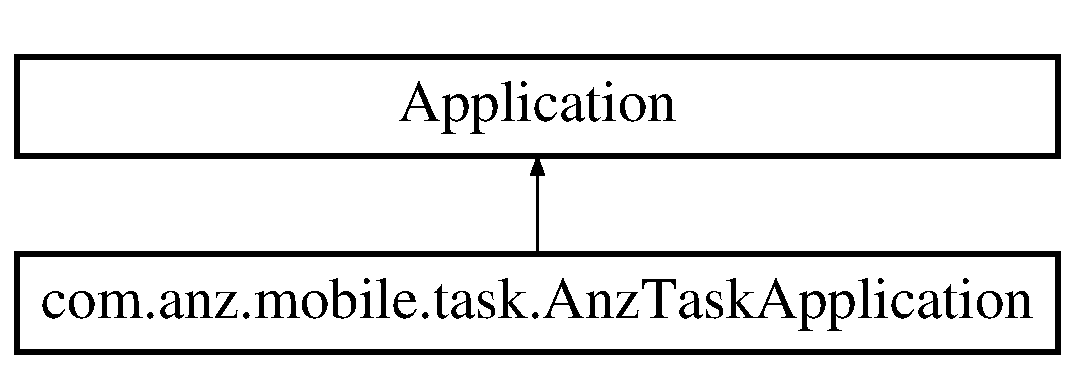
\includegraphics[height=2.000000cm]{classcom_1_1anz_1_1mobile_1_1task_1_1_anz_task_application}
\end{center}
\end{figure}
\subsection*{Public Member Functions}
\begin{DoxyCompactItemize}
\item 
\hypertarget{classcom_1_1anz_1_1mobile_1_1task_1_1_anz_task_application_a162b6099a5b53bf44590cf6c2f83e041}{void {\bfseries on\+Create} ()}\label{classcom_1_1anz_1_1mobile_1_1task_1_1_anz_task_application_a162b6099a5b53bf44590cf6c2f83e041}

\end{DoxyCompactItemize}


The documentation for this class was generated from the following file\+:\begin{DoxyCompactItemize}
\item 
/\+Users/\+Ning/\+Desktop/\+Anz\+Task/\+Android/\+Project/\+Anz\+Task/app/src/main/java/com/anz/mobile/task/Anz\+Task\+Application.\+java\end{DoxyCompactItemize}

%--- End generated contents ---

% Index
\newpage
\phantomsection
\addcontentsline{toc}{chapter}{Index}
\printindex

\end{document}
